\chapter{Tecnologie}
In questo capitolo verranno descritte le attività preliminari per la realizzazione di questo progetto, le tecnologie utilizzate
unitamente alle motivazioni legate all'uso di questi sistemi rispetto ad altri.

\section{Strutture dati gerarchiche}
Le tabelle di un database relazione non sono gerarchiche (come nel XML), ma sono delle semplici liste piatte. I dati gerarchici sono 
constituiti da relazioni padre-figlio che non possono essere rappresentate in modo naturale nelle tabelle dei database relazionali.
In questo caso, i dati gerarchici sono una collezione di informazioni dove ogni item ha un solo padre e nessuno o più figli
(ad eccezione del nodo radice che non ha un nodo padre); questo genere di rappresentazione delle informazioni può essere trovato in 
diversi ambiti di applicazione di un database, incluse discussioni su forum e mailing list, grafici di organizzazione di un business, 
categorie per gestire contenuti e categorie di prodotti. 

\begin{figure}[H]
	\label{fig:Hde}
	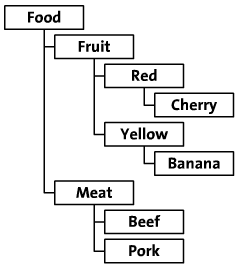
\includegraphics[scale=0.45]{images/Hierarchical_Data_ex.PNG}
	\caption{Esempio di una gestione di dati in modo gerarchico}
\end{figure}

Ci sono differenti modelli per poter gestire dati in modo gerarchico, i più importanti che sono stati presi in considerazione sono i 
seguenti:

\newpage

\subsection{The adjacency list model}
Il primo approccio, e quello di più semplice implementazione, qui descritto è chiamato \textit{‘adjacency list model} o metodo ricorsivo;
è definito tale perchè per funzionare necessita solo di una funzione che itera per tutto l'albero.

In questo modello, ogni item (nodo dell'albero) nella tablla contiene un puntatore al suo item padre; invece il nodo radice avrà un puntatore a un valore
NULL per l'item padre.

\begin{figure}[ht!]
    \centering
	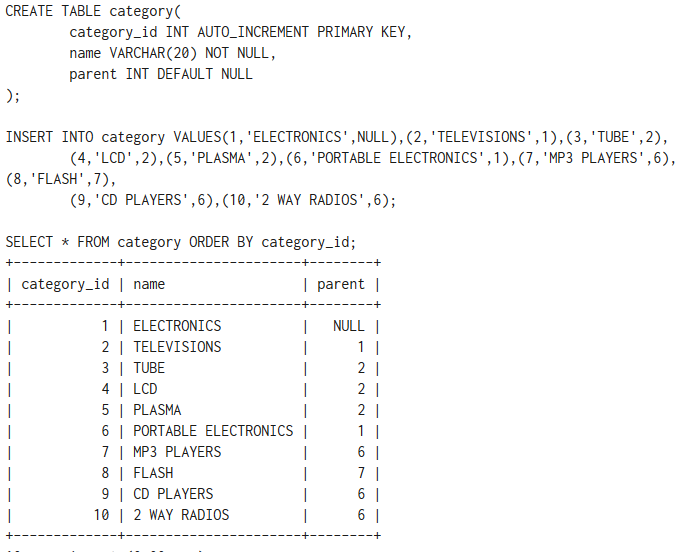
\includegraphics[scale=0.75]{images/Adjacency_list_model_table.PNG}
	\caption{Esempio di una tabella per gestire dati in modo gerarchico secondo l' adjacency list model }
\end{figure}
 
Il vantaggio di usare questo modello sta nella sua semplicità di costruzione sopratutto a livello di codice client-side, 
e di restituzione dei figli di un nodo. Mentre diventa problematico se si lavora in puro SQL e nella maggior parte dei linguaggi di 
programmazione, è lento e poco efficente, perchè è necessaria una query per ogni nodo dell'albero, e visto che ogni query impiega 
un certo periodo di tempo, questo rende la funzione molto lente quando si lavora con alberi di grandi dimensioni.
Inoltre molti linguaggi non sono ottimizzati per funzioni ricorsive. Per ogni nodo, la funzione inizia una nuova istanza di se stessa,
ogni istanza occupa una porzione di memoria e impiega un certo tempo per inizializzarsi, e più grande è l'albero e più questo 
processo sarà portato a termine in maggior tempo.

\newpage

\subsection{The Nested set model}
Il secondo approccio che viene proposto è il \textit{Nested set model}, che permette di osservare la gerarchia in un modo diverso, non 
come nodi e linee, ma come container innestati.

\begin{figure}[ht!]
    \centering
	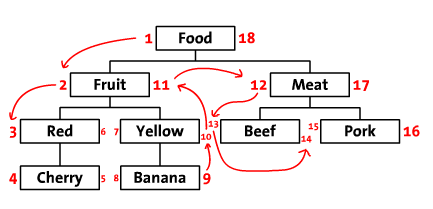
\includegraphics[scale=0.6]{images/Nested_Tree_Model_ex.PNG}
	\caption{Esempio di una gestione di dati in modo gerarchico secondo il Nested set model}
\end{figure}

La gerarchia dei dati viene rappresentata nella tabella attraverso l'uso degli attributi 'left' e 'right' per rappresentare l'annidamento
dei nodi (il nome delle colonne: left e right, hanno significati speciali in SQL; per questo motivo si identificano questi campi con i 
nomi 'lft' e 'rght'). 
Ogni nodo dell'albero viene visitato due volte, assegnando i valori in ordine di visita, e in entrambe le visite. Quindi vengono 
associati ad ogni nodo due numeri, memorizzato come due attributi. 
I valori di left e right sono determinati come segue: si inizia a numerare a partire dal lato più a sinistra di ogni nodo e si continua 
verso destra. Lavorando con un albero, si parte da sinistra e si continua verso destra, un livello alla volta, scendendo per ogni
nodo i suoi figli, assegnando i valori al campo left, prima di assegnare un valore al campo right, e successivamente si continua verso 
destra.
Questo approccio è chiamato Modified preorder tree traversal algorithm.

A prima vista questo approccio può sembrare più complicato da comprendere rispetto all'adjacency list model, ma quest'utlimo metodo è
molto più veloce quando si vuole recuperare i nodi, visto che basta una query, mentre più lento per operazioni di aggiornamento e 
cancellazione dei nodi; in quest ultimo il grado di complicatezza dell'operazione è determinato dal nodo che si vuole cancellare, a 
partire dal caso più semplice, il nodo foglia (nodo senza figli) fino al caso più complicato, quando si vuole cancellare il nodo radice.

\begin{figure}[ht!]
    \centering
	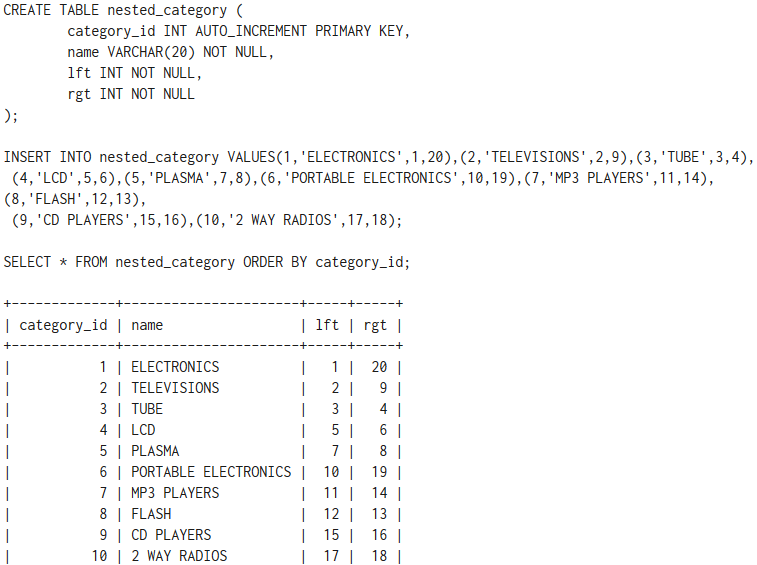
\includegraphics[scale=0.6]{images/Nested_Tree_Model_table.PNG}
	\caption{Esempio di una tabelle per la gestione di dati in modo gerarchico secondo il Nested set model}
\end{figure}


\section{Sistemi di raccomandazione}